\section{Introduction}
There exist different types of stable coins which are categorized to backed stablecoins and algorithmic mechanism stablecoins. Backed stablecoins could be directly backed by a fiat currency or indirectly backed by another volatile asset (for example backed by ETH). In this type one solution to mitigate the volatility is to overcollateralize the deposited asset. In this paper, we propose an imaginary stablecoin model that uses indirectly backed mechanism namely RBcoin (stands from Red Black coin).

RBcoin is a Decentralized Application (DApp) which holds ETH and issue tokens. The DApp determines how much ETH is equivalent to \$1.50 USD using the current exchange rate, provided to the DApp by a trusted third party oracle, and Alice deposits this amount of ETH into the DApp. The DApp issues Alice two places in a line — each place is a transferable token Red token and Black token. At some future time, the holder of the first place in line can redeem up to \$1.00 USD worth of the deposited ETH at the going exchange rate, and the holder of the second place in line gets any remaining ETH. Alice will transfer the first place in line (as a stable coin called Red coin) to Bob for \$1.00 and will hold or sell the second place in line (Black coin). When Bob redeems the Red coin, it will be worth \$1 USD in ETH when the entire deposit of ETH is worth more than \$1 USD. If the exchange rate drops enough, the entire deposit will be worth less than \$1 USD — Bob will get all of the deposit and the holder of the second place in line will get nothing.

The price of ETH to USD is volatile and there is a chance that ETH drops a lot and results in a bad situation in which our Red stable coin worth lesser than \$1. In this paper, we analyze the impact of different design factors of the RBcoin model on the failure rate of stability of Red coin. Also, we will talk about features of RBcoins like fungibility, governance, balance mechanism for demand and supply, and implications of regulation on these types of stable coins. 
\section{Analysis on RBcoins}

In this section we analyze stability of RBcoin by changing design and estimation paramethers. We change each factor one by one and check the results of these changes on Redcoin and Blackcoin price estimations.

We use Geometric Brownian Motion (GBM) along with Monte Carlo method for our ETH/USD price simulations. The number of Monte-Carlo method simulations is 1000 and default paramethers used for each simulation is \$1.5 collateral amount in ETH and 100 days for estimation. In some parts we will change these default paramethers to see the result of changes.

We use data on the price of ETH/USD from coingecko and the period of our data is from 1 Januery 2018 to \textcolor{red}{4 May 2020}.

Figure 1 shows the result of Monte Carlo simulations on ETH/USD price for 100 future days.
\begin{figure} [H]
\centering
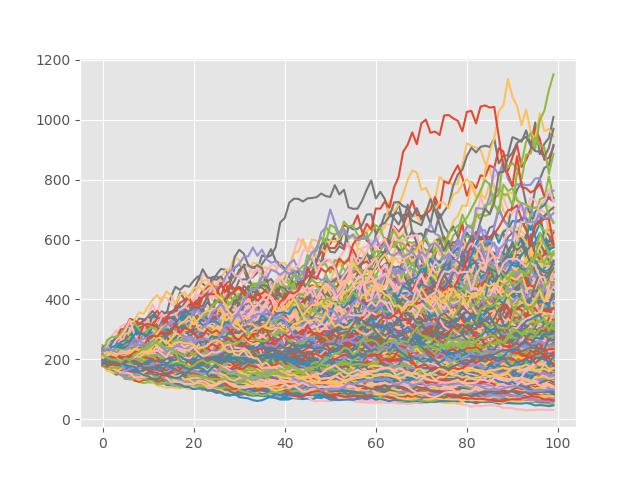
\includegraphics[width=8cm]{Monte-Carlo}
\caption{Monte Carlo forcasts of ETH/USD for 100 days}
\end{figure}
Figure 2 shows the histogram ETH/USD output results of 1000 different simulations of Monte-Carlo method of ETH/USD prices in day 100 of simulations. It supposed to be a Log-Normal distribution.
\begin{figure} [H]
\centering
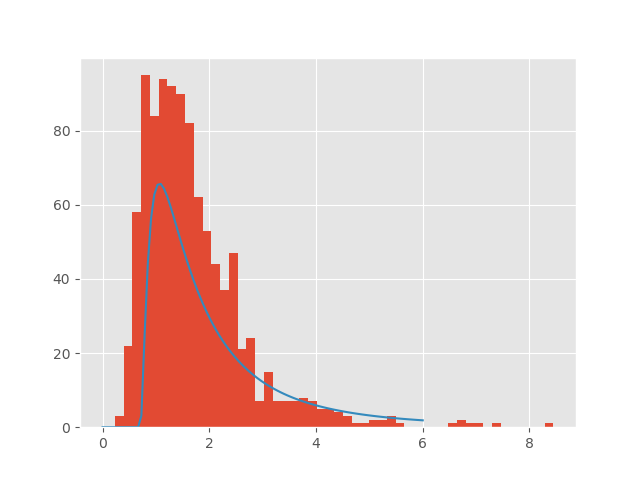
\includegraphics[width=8cm]{outputs}
\caption{Histogram of ETH prices in day 100 of simulations}
\end{figure}

The mean of all 1000 Monte-Carlo simulations for day 100 of estimations is \textcolor{red}{1.6999126476323942} and the standard deviation is \textcolor{red}{0.9957392528773387}.

Figure 3 is log of outputs in figure 2 to show that the distrubution of log of outputs is a normal shape distribution.

\begin{figure} [H]
\centering
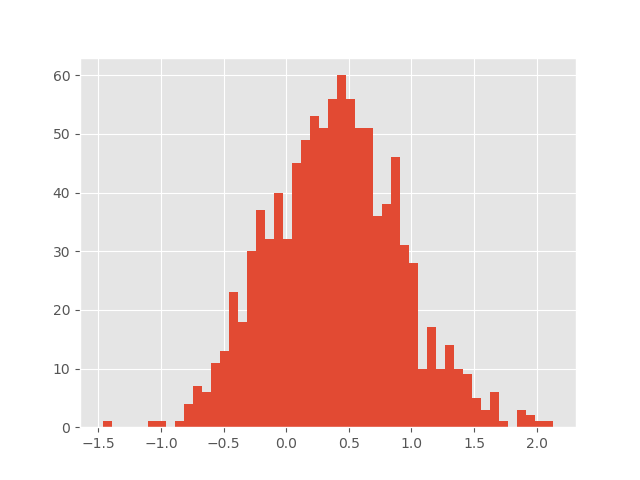
\includegraphics[width=8cm]{normaloutpts}
\caption{Histogram of log of ETH prices in day 100 of simulations}
\end{figure}


In next sections we will analyze the outputs of Red and Black coin for each set of simulations and then analyze the impact of each design factor on Red and Black coins.

\subsection{Impact of ETH/USD volatility on the Red and Black coin}

The price of Ether is volatile from its Initial Coin Offering (ICO) until today. The highest historical price of ETH was \$1,360 in early 2018 but today's price of ETH on May 4th is \$214. 
ETH price change may have different impacts on the price of our Red and Black coin on RBcoin DApp. In Table 1 we show the impact of changes of ETH/USD on Blackcoin and Redcoin.



% Please add the following required packages to your document preamble:
% \usepackage[table,xcdraw]{xcolor}
% If you use beamer only pass "xcolor=table" option, i.e. \documentclass[xcolor=table]{beamer}
\begin{table}[H]
\begin{tabular}{l|l|l|}
\cline{2-3}
                                                                & {\color[HTML]{000000} Red Coin} & Black Coin                  \\ \hline
\multicolumn{1}{|l|}{{\color[HTML]{000000} Big drop on ETH}}    & \textless{}\$1                  & Zero                        \\ \hline
\multicolumn{1}{|l|}{{\color[HTML]{000000} Little drop on ETH}} & \$1                             & Much lower than \$0.5       \\ \hline
\multicolumn{1}{|l|}{Without changes}                           & \$1                             & \$0.5                       \\ \hline
\multicolumn{1}{|l|}{Little rise on ETH}                        & \$1                             & Much higher than \$0.5      \\ \hline
\multicolumn{1}{|l|}{Big rise on ETH price}                     & \$1                             & Much Much higher than \$0.5 \\ \hline
\end{tabular}
\caption{Impact of ETH volatility on RBcoin}
\label{tbl1}
\end{table}

So naturally, the question will arise: How often each scenario will occur? 

To answer this question we analyze the results of day 100 simulations for three different scenarios as below:


\subsubsection{Significant drop on ETH price}
The worst-case scenario is when the price of ETH in the US dollar drops sharply. So the value of deposited ETH in our RBcoin DApp is bellow \$1. In this situation, the Black coin has zero price and the Red coin is worth bellow \$1 and not yet pegging a dollar. 

In one experiment \textcolor{red}{237} outcomes out of 1000 simulations have results bellow \$1 which tells us the probability of instability on RBcoin is about 23.7\%. The mean for the Redcoins in this situation is \textcolor{red}{0.7683783229826656}. 

\subsubsection{A little drop on ETH price}
In this situation, the Redcoin price is \$1. Because the ETH price is dropped and consequently the equivalent value of the deposited amount of ETH in the dollar is dropped so the value of the Black coin is dropped a lot.

In an experiment \textcolor{red}{302} simulations out of 1000 results in a bit drop on ETH after 100 days. In this scenario the mean of these \textcolor{red}{302} outcomes for the Black coin is \textcolor{red}{0.2458290144866682} with the standard deviation of \textcolor{red}{0.1366094047375821}. 

\subsubsection{Rise in ETH price}
If the price of ETH in USD goes up the Redcoin will be stable so its value will be \$1. Therefore because ETH price goes up and the Redcoin is stable and the value of deposited ETH is equal to the summation of Redcoin and Blackcoin value, the value of the Black coin will go up on a higher rate compared to the changes in ETH/USD. For example, assume a situation in which the price of ETH in dollar changes $\alpha$ percents and Alice (who deposited ETH on RBcoin DApp) deposited \$1.5 so the collateral amount is \$1.5. So we have:

\[Value of Deposited ETH = Black coin + Red coin\]

By assuming that the value of deposited ETH will not drop bellow \$1 the value of Red coin is \$1. And because of $\alpha$ percent changes in ETH value in the dollar, the value of Deposited ETh is 1.5 * $\alpha$.

\[Value of Black coin = 1.5\alpha - 1\]

If Bob bought Black coin from Alice on day 0, he paid \$0.5 for the Black coin. In this situation for calculation return ratio for Bob on day 100 we have :

\begin{equation} \label{eq1}
\begin{split}
Return & = \frac{1.5\alpha - 1}{0.5} \\
 & = 3\alpha - 2
\end{split}
\end{equation}

Using Equation \ref{eq1} and the fact that che changes on ETH price in dollar is $\alpha$ percent we can define leverage ratio for investment on Black coin as:

\begin{equation} \label{eq2}
\begin{split}
Leverage Ratio & = \frac{3\alpha - 2}{\alpha} \\
 & = 3- \frac{2}{\alpha}
\end{split}
\end{equation}

Regarding Equation \ref{eq2} Leverage Ratio of the Black coin position will be increased when ETH value in the dollar goes up.

So the leverage ratio of the Black coin is depending on the change of ETH price after the contract. Using this equation for $\alpha$ equals to $\frac{2}{3} $ the Leverage ratio becomes zero. The reason is that if the ETH price drops 33.33\% then the value of deposited ETH is \$1 and so the Black coin price will be zero. 

Another interesting fact using Equation \ref{eq2} is that the highest Leverage ratio in the Black coin position will be 3 and it is when the price of ETH goes up a lot compared to the time of the contract.

In the previous part, we analyze the leverage ratio of the Black coin assuming $\alpha$ percent changes on ETH price. In this part, we combine the results of our Monte-Carlo simulations which shows ETH price changes estimations and the Leverage Ratio formula. 
In an experiment of 1000 simulations and using Equation \ref{eq2} we analyze two different situations. In first we use simulation outcomes in which the resulted amount of ETH on day 100 is higher than \$1.5 (which means $\alpha$ is higher than 1). In this situation the mean of all resulted Leverage Ratios are \textcolor{red}{2.0756085371941726} with standard deviation of \textcolor{red}{0.24043476162253544}. In another scenario, we pick all outcomes with resulted in ETH higher than \$1 (which means the value of the Black coin is non-zero). In this scenario  the mean of all resulted Leverage Ratios are \textcolor{red}{1.8120987004369604} with standard deviation of \textcolor{red}{0.4117814399925659}.

All of this description has an assumption that Alice (the deposited \$1.5 as collateral). If Alice decides to deposit a higher amount as collateral the Leverage ratio will be decreased and it is logical because Alice takes a lower risk for lower reward.

\textcolor{green}{Maybe some description needed???}.

\subsection{Impact of Over-Collaterallization Ratio}
Stablecoins that are indirectly backed by crypto-assets like ETH are prone to a risk of the volatility of the asset. This risk is addressed by over-collateralization of the volatile asset. For example, in DAI stablecoin the collateralization ratio is 1.5 like our imaginary model RBcoin. After depositing that amount the depositor receives two places in line. A stablecoin (Red coin) and a leveraged coin (Black coin). But there is a debate on this ratio. Does 1.5 over-collateralization ratio is high enough to mitigate the risk of volatility? Could the over-collateralization ratio be lower than this amount to help the new depositors?
In this section, we analyze the impact of the over-collateralization ratio on the stability of RBcoin DApp and the value of Red and Black coin.

In Table \ref{tbl2} we analyze the outcomes for different amount of collateral by depositor.
\begin{table}[H]
\begin{tabular}{l|l|l|l|l|l|}
\cline{2-6}
                                                                                                            & {\color[HTML]{000000} \$1.05} & \$1.25 & \$1.5  & \$1.75 & \$2    \\ \hline
\multicolumn{1}{|l|}{{\color[HTML]{000000} Mean of outcomes}}                                               & 1.1871                        & 1.4194 & 1.7494 & 1.9787 & 2.2588 \\ \hline
\multicolumn{1}{|l|}{{\color[HTML]{000000} Stdev of outcomes}}                                              & 0.7160                        & 0.7853 & 1.0569 & 1.1370 & 1.3264 \\ \hline
\multicolumn{1}{|l|}{\begin{tabular}[c]{@{}l@{}}Number of cases\\ with zero blackcoins\end{tabular}}        & 490                           & 343    & 229    & 164    & 90     \\ \hline
\multicolumn{1}{|l|}{\begin{tabular}[c]{@{}l@{}}Average of Redcoins\\ bellow \$1\end{tabular}}              & 0.6841                        & 0.7298 & 0.7688 & 0.7841 & 0.7884 \\ \hline
\multicolumn{1}{|l|}{\begin{tabular}[c]{@{}l@{}}Mean of Leverage\\ for non-zero Black\\ coins\end{tabular}} & 1.6496                        & 1.7236 & 1.8396 & 1.9189 & 1.9765 \\ \hline
\end{tabular}
\caption{Impact of Collateral Ratio on RBcoin}
\label{tbl2}
\end{table}

\subsection{Impact of simulation days in RBcoin analysis}
One of the parameters in our experiments is the day of simulations. It is obvious that by increasing the number of days of predictions the standard deviation of results will be increased. Therefore by using Geometric Brownian Motion and Monte-Carlo because of increasing standard deviation the results of the output depend on the total estimation of these models. It means if these methods overall predict that the price will go up then by increasing the day of prediction the average price results on last day will be increased and vice versa if the overall estimation is that the price will drop then by increasing the days of the simulation the average of the results prices on last day will be dropped.

In Table \ref{tbl3} we analyze some outcomes of the Monte-Carlo method for different days of predictions.

\begin{table}[H]
\begin{center}
\begin{tabular}{l|l|l|l|l|}
\cline{2-5}
                                                                                                            & {\color[HTML]{000000} 100} & 200    & 300    & 365    \\ \hline
\multicolumn{1}{|l|}{{\color[HTML]{000000} Mean of outcomes}}                                               & 1.6320                     & 1.9082 & 2.1779 & 2.2390 \\ \hline
\multicolumn{1}{|l|}{{\color[HTML]{000000} Stdev of outcomes}}                                              & 0.9272                     & 1.7857 & 2.3276 & 3.4074 \\ \hline
\multicolumn{1}{|l|}{\begin{tabular}[c]{@{}l@{}}Number of cases\\ with zero blackcoins\end{tabular}}        & 251                        & 318    & 307    & 430    \\ \hline
\multicolumn{1}{|l|}{\begin{tabular}[c]{@{}l@{}}Average of Redcoins\\ bellow \$1\end{tabular}}              & 0.7311                     & 0.6380 & 0.5771 & 0.5542 \\ \hline
\multicolumn{1}{|l|}{\begin{tabular}[c]{@{}l@{}}Mean of Leverage\\ for non-zero Black\\ coins\end{tabular}} & 1.8033                     & 1.9466 & 2.0047 & 2.0667 \\ \hline
\end{tabular}
\caption{Impact of simulation days in Analysis}
\label{tbl3}
\end{center}
\end{table}

\subsection{Impact of early Liquidation}
This stability mechanism might enable a third-party to trigger a redemption (for a fee) if they notice a deposit is close to losing more value than the face value of the coins (before the coin holder does). Note that while allowing third parties to trigger a redemption seems like a sensible service, if the coin holders are not monitoring the situation, they will end up holding ETH, instead of an AliceCoin, which is still losing value. Thus this mechanism does not protect holders of the stablecoin at all --- it is really only about maintaining the reputation of the stablecoin. The stablecoin can claim it has never broken its peg to the dollar but it is an illusion, because as soon as it is about to lose value, it turns back into its collateral and then loses values under the name of the collateral instead of the stablecoin. If the holder isn’t paying attention, they actually lose more by having it triggered than they would breaking the buck.